\chapter{TASK\_7.}

\textbf{Цель работы:}

\begin{itemize} 
	\item Изучать и реализовать взаимодействие между серверами.
	\item Изучать и реализовать дочерние процессы.
	\item Изучать и реализовать process.argv.
\end{itemize}

\textbf{Задание 1}

Создать сервер А. На стороне сервера хранится файл с содержимым в формате JSON. При получении запроса на /insert/record идёт добавление записи в файл. При получении запроса на /select/record идёт получение записи из файла. Каждая запись хранит информацию о машине (название и стоимость).

Создать сервер Б. На стороне сервера хранится файл с содержимым в формате JSON. Каждая запись в файле хранит информацию о складе и массиве машин, находящихся на данном складе. То есть каждая запись хранит в себе название склада (строку) и массив названий машин (массив строк). При получении запроса на /insert/record идёт добавление записи в файл. При получении запроса на /select/record идёт получение записи из файла.

Создать сервер C. Сервер выдаёт пользователю страницы с формами для ввода информации. При этом сервер взаимодействует с серверами А и Б. Реализовать для пользователя функции:

создание нового типа машины
получение информации о стоимости машины по её типу
создание нового склада с находящимися в нём машинами
получение информации о машинах на складе по названию склада
Реализовать удобный для пользователя интерфейс взаимодействия с системой (использовать поля ввода и кнопки).

\begin{lstlisting}[caption=Код программы. TASK\_7. Сервер A]
	"use strict";

// импорт библиотеки
const express = require("express");
const fs = require("fs");


// запускаем сервер
const app = express();
const port = 5003;
app.listen(port);
console.log("Server on port " + port);

// заголовки для ответа
app.use(function (req, res, next) {
	res.header("Cache-Control", "no-cache, no-store, must-revalidate");
	res.header("Access-Control-Allow-Headers", "Origin, X-Requested-With, Content-Type, Accept");
	res.header("Access-Control-Allow-Origin", "*");
	next();
});

// Загрузка тела.
function loadBody(request, callback) {
	let body = [];
	request.on('data', (chunk) => {
		body.push(chunk);
	}).on('end', () => {
		body = Buffer.concat(body).toString();
		callback(body);
	});
}

// Приём запроса.
app.post("/insert/record", function (request, response) {
	loadBody(request, function (body) {
		// Получаем данные.
		const obj = JSON.parse(body);
		const type = obj.type;
		const price = obj.price;

		// Открываем файл и парсим.
		const fileName = "data_car.json";
		const objInfo = fs.readFileSync(fileName, "utf-8");
		const infoJson = JSON.parse(objInfo);
		let answer = "Model is exist!";

		let flag = true;
		// Ищем модель.
		for (let i in infoJson) {
			if (infoJson[i].type === type) {
				// console.log(infoJson[i]);
				flag = false;
				break;
			}
		}

		// Добавляем в файл информацию,
		// Если такой модели еще нет.
		if (flag) {
			infoJson.push({ type, price })
			fs.writeFileSync(fileName, JSON.stringify(infoJson, null, 4));
			answer = "Model add";
		}

		response.end(JSON.stringify({ answer: answer }));
	});
});

// Приём запроса.
app.post("/select/record", function (request, response) {
	loadBody(request, function (body) {
		// Получаем данные.
		const obj = JSON.parse(body);
		const type = obj.type;

		// Открываем файл и парсим.
		const fileName = "data_car.json";
		const objInfo = fs.readFileSync(fileName, "utf-8");
		const infoJson = JSON.parse(objInfo);

		// Ответ пользователю.
		let answer = "Model does not!";

		// Ищем модель.
		for (let i in infoJson) {
			if (infoJson[i].type === type) {
				// console.log(infoJson[i]);
				answer = infoJson[i];
				break;
			}
		}

		response.end(JSON.stringify({ answer: JSON.stringify(answer) }));
	});
});
\end{lstlisting}

\begin{lstlisting}[caption=Код программы. TASK\_7. Сервер B]
	"use strict";

// импорт библиотеки
const express = require("express");
const fs = require("fs");


// запускаем сервер
const app = express();
const port = 5002;
app.listen(port);
console.log("Server on port " + port);

// заголовки для ответа
app.use(function (req, res, next) {
	res.header("Cache-Control", "no-cache, no-store, must-revalidate");
	res.header("Access-Control-Allow-Headers", "Origin, X-Requested-With, Content-Type, Accept");
	res.header("Access-Control-Allow-Origin", "*");
	next();
});

// Загрузка тела.
function loadBody(request, callback) {
	let body = [];
	request.on('data', (chunk) => {
		body.push(chunk);
	}).on('end', () => {
		body = Buffer.concat(body).toString();
		callback(body);
	});
}

// Приём запроса.
app.post("/insert/record", function (request, response) {
	loadBody(request, function (body) {
		// Получаем данные.
		const obj = JSON.parse(body);
		const stock_name = obj.stock_name;
		const car_array_str = obj.car_array;

		// Открываем файл и парсим.
		const fileName = "data_stock.json";
		const objInfo = fs.readFileSync(fileName, "utf-8");
		const infoJson = JSON.parse(objInfo);
		let answer = "Stock is exist!";

		let flag = true;
		// Ищем склад.
		for (let i in infoJson) {
			if (infoJson[i].stock_name === stock_name) {
				// console.log(infoJson[i]);
				flag = false;
				break;
			}
		}

		// Добавляем в файл информацию,
		// Если такой модели еще нет.
		if (flag) {
			let car_array = car_array_str.split(" ");
			infoJson.push({ stock_name, car_array })
			fs.writeFileSync(fileName, JSON.stringify(infoJson, null, 4));
			answer = "Model add";
		}

		response.end(JSON.stringify({ answer: answer }));
	});
});

// Приём запроса.
app.post("/select/record", function (request, response) {
	loadBody(request, function (body) {
		// Получаем данные.
		const obj = JSON.parse(body);
		const name_stock_find = obj.name_stock_find;

		// Открываем файл и парсим.
		const fileName = "data_stock.json";
		const objInfo = fs.readFileSync(fileName, "utf-8");
		const infoJson = JSON.parse(objInfo);

		// Ответ пользователю.
		let answer = "Model does not!";

		// Ищем модель.
		for (let i in infoJson) {
			if (infoJson[i].stock_name === name_stock_find) {
				// console.log(infoJson[i]);
				answer = infoJson[i];
				break;
			}
		}

		response.end(JSON.stringify({ answer: JSON.stringify(answer) }));
	});
});
\end{lstlisting}

\begin{lstlisting}[caption=Код программы. TASK\_7.Сервер C]
	"use strict";

// импорт библиотек
const express = require("express");
const request = require("request");
const fs = require("fs");

const ENCODING = "utf-8"

// запускаем сервер
const app = express();
const port = 5000;
app.listen(port);
console.log(`Server on port ${port}`);

// Отправка статических файлов.
const way = __dirname + "/static";
app.use(express.static(way));

// заголовки в ответ клиенту
app.use(function (req, res, next) {
	res.header("Cache-Control", "no-cache, no-store, must-revalidate");
	res.header("Access-Control-Allow-Headers", "Origin, X-Requested-With, Content-Type, Accept");
	res.header("Access-Control-Allow-Origin", "*");
	next();
});

// функция для отправки POST запроса на другой сервер
function sendPost(url, body, callback) {
	// задаём заголовки
	const headers = {};
	headers["Cache-Control"] = "no-cache, no-store, must-revalidate";
	headers["Connection"] = "close";
	// отправляем запрос
	request.post({
		url: url,
		body: body,
		headers: headers,
	}, function (error, response, body) {
		if (error) {
			callback(null);
		} else {
			callback(body);
		}
	});
}

app.get("/", (_request, response) => {
	const fileContent = fs.readFileSync("static/" + "index.html", ENCODING);
	response.end(fileContent);
});

// принимаем GET запрос и отправляем POST запрос на другой сервер
app.get("/set_info_car/", (request, response) => {
	const type = request.query.field_type_car;
	const price = request.query.field_price_car;

	sendPost("http://localhost:5003/insert/record", JSON.stringify(
		{ type, price }
	), function (answerString) {
		const answerObject = JSON.parse(answerString);
		const answer = answerObject.answer;
		response.end("Answer: " + answer);
	});
});

app.get("/get_info_car/", (request, response) => {
	const type = request.query.field_type_car_find;

	sendPost("http://localhost:5003/select/record", JSON.stringify(
		{ type }
	), function (answerString) {
		const answerObject = JSON.parse(answerString);
		const answer = answerObject.answer;
		response.end("Answer: " + answer);
	});
});

// принимаем GET запрос и отправляем POST запрос на другой сервер
app.get("/set_info_stock/", (request, response) => {
	const stock_name = request.query.field_stock_name;
	const car_array = request.query.field_car_array;

	sendPost("http://localhost:5002/insert/record", JSON.stringify(
		{ stock_name, car_array }
	), function (answerString) {
		const answerObject = JSON.parse(answerString);
		const answer = answerObject.answer;
		response.end("Answer: " + answer);
	});
});

app.get("/get_info_stock/", (request, response) => {
	const name_stock_find = request.query.field_name_stock_find;

	sendPost("http://localhost:5002/select/record", JSON.stringify(
		{ name_stock_find }
	), function (answerString) {
		const answerObject = JSON.parse(answerString);
		const answer = answerObject.answer;
		response.end("Answer: " + answer);
	});
});
\end{lstlisting}

\textbf{Задание 2}

Написать скрипт, который принимает на вход число и считает его факториал. Скрипт должен получать параметр через process.argv.

Написать скрипт, который принимает на вход массив чисел и выводит на экран факториал каждого числа из массива. Скрипт принимает параметры через process.argv.

При решении задачи вызывать скрипт вычисления факториала через execSync.

\begin{lstlisting}[caption=Код программы. TASK\_7. Задание 2. Главный процесс]
	"use strict";
	
	// импортируем библиотеку
	const execSync = require('child_process').execSync;
	
	const MY_ARG = 2
	const OPTIONS = { encoding: 'utf8' };
	
	// Функция, для считывания аргументов
	// Переданных в командной строке.
	function readArgv(array) {
		let i = MY_ARG;
	
		while (process.argv[i])
			array.push(parseInt(process.argv[i++]));
	
		return array;
	}
	
	// Функция, вызывающая дочерний процесс
	// Для каждого элемента из массива array.
	// Дочерний процесс в свою очередь
	// Считает факториал числа.
	function arrayFactorial(array) {
		let cmd;
	
		for (let i in array) {
			cmd = `node factorial ${array[i]}`
			console.log(execSync(cmd, OPTIONS))
		}
	}
	
	
	function main() {
		let array = [];
		readArgv(array);
		arrayFactorial(array);
	}
	
	main();
\end{lstlisting}


\begin{lstlisting}[caption=Код программы. TASK\_2. Задание 2. Дочерний процесс.]
"use strict";

// Функция, которая вычисляет факториал
// Числа, переданного аргументом командной строки.
function factorial() {
	let num = parseInt(process.argv[2]);
	let result = 1;

	for (let i = 1; i < num; i++)
		result *= i;

	console.log(result);
}

factorial();
\end{lstlisting}

\textbf{Вывод:}

\begin{itemize} 
	\item Мы изучили и реализовали взаимодействие между серверами.
	\item Изучили и реализовали дочерние процессы.
	\item Изучили и реализовали process.argv.
\end{itemize}


\textbf{Пример работы:}

\begin{figure}[ht!]
	\centering{
		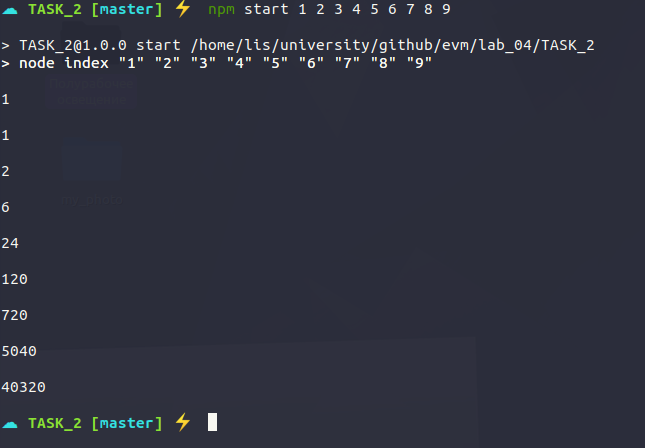
\includegraphics[width=0.9\textwidth]{img/1.png}
		\caption{Пример работы программы}}
\end{figure}


\begin{figure}[ht!]
	\centering{
		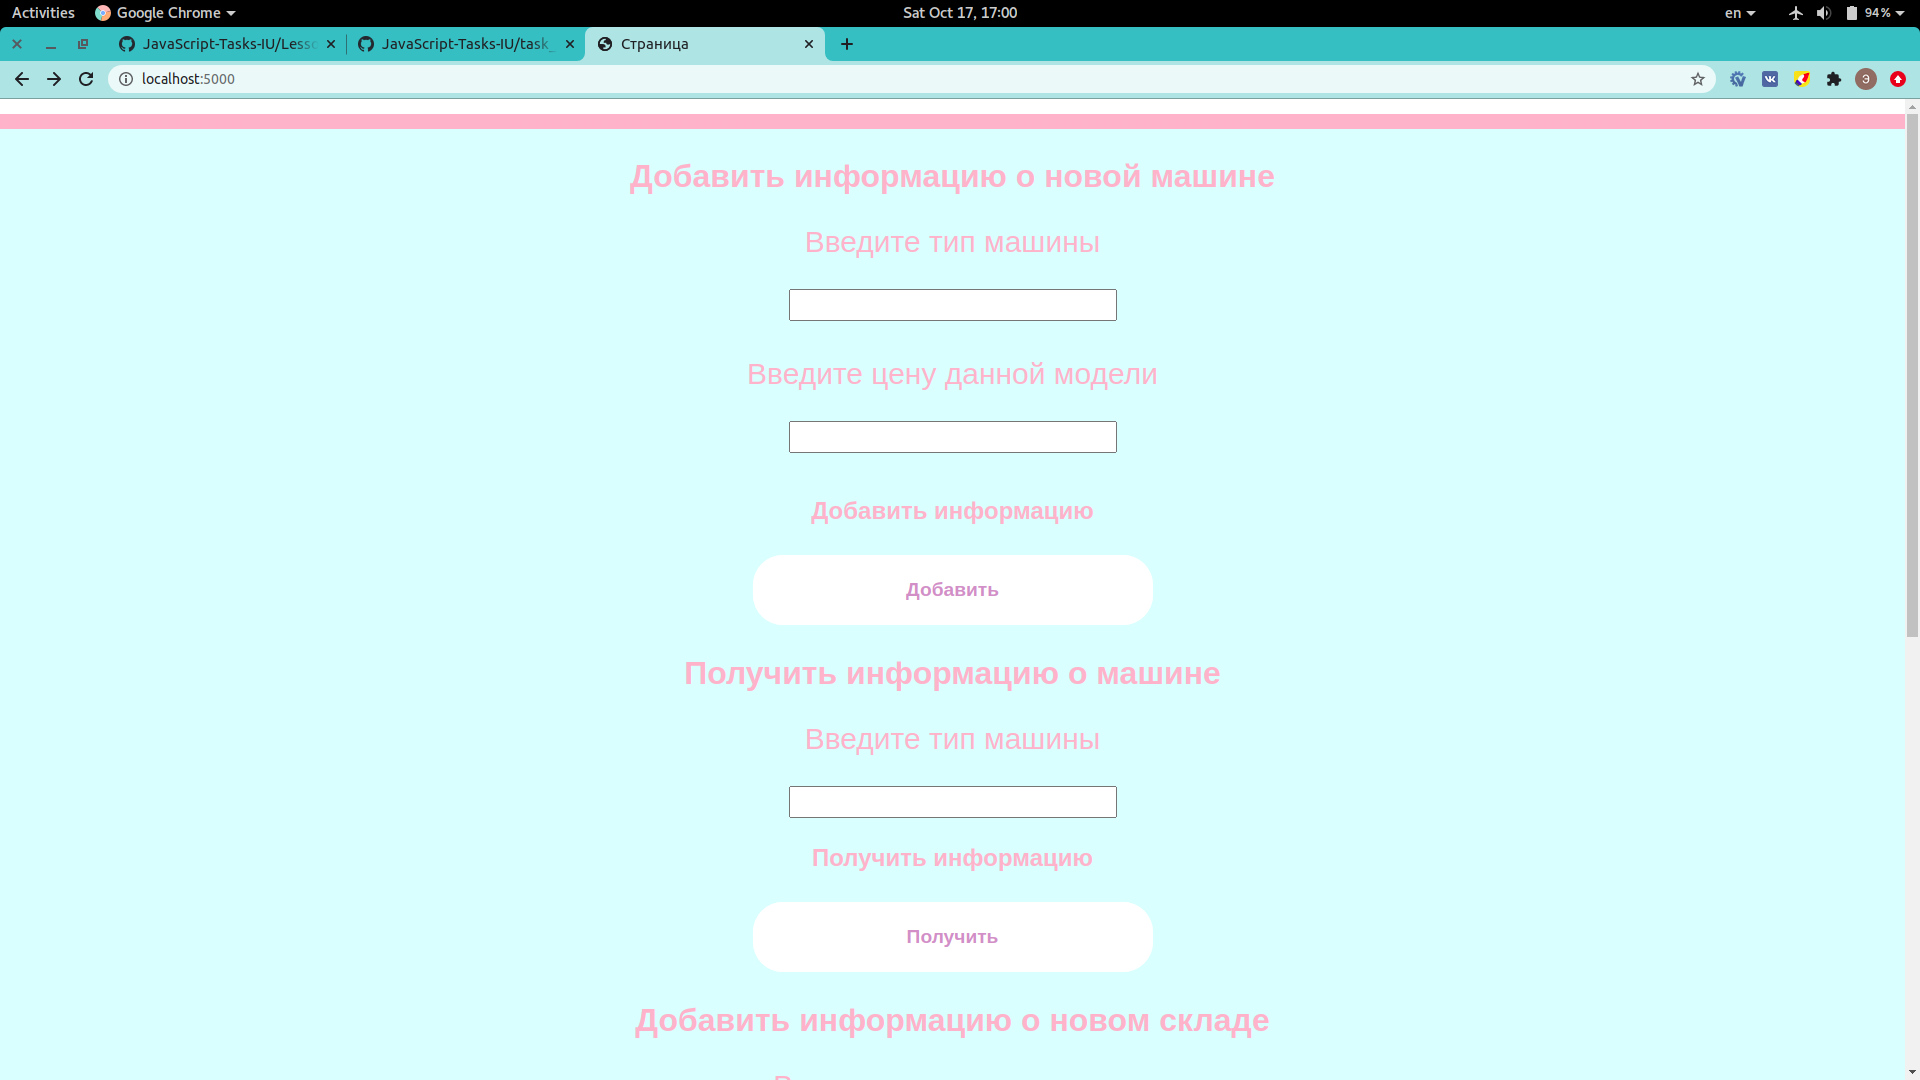
\includegraphics[width=0.9\textwidth]{img/2.png}
		\caption{Пример работы программы}}
\end{figure}


\begin{figure}[ht!]
	\centering{
		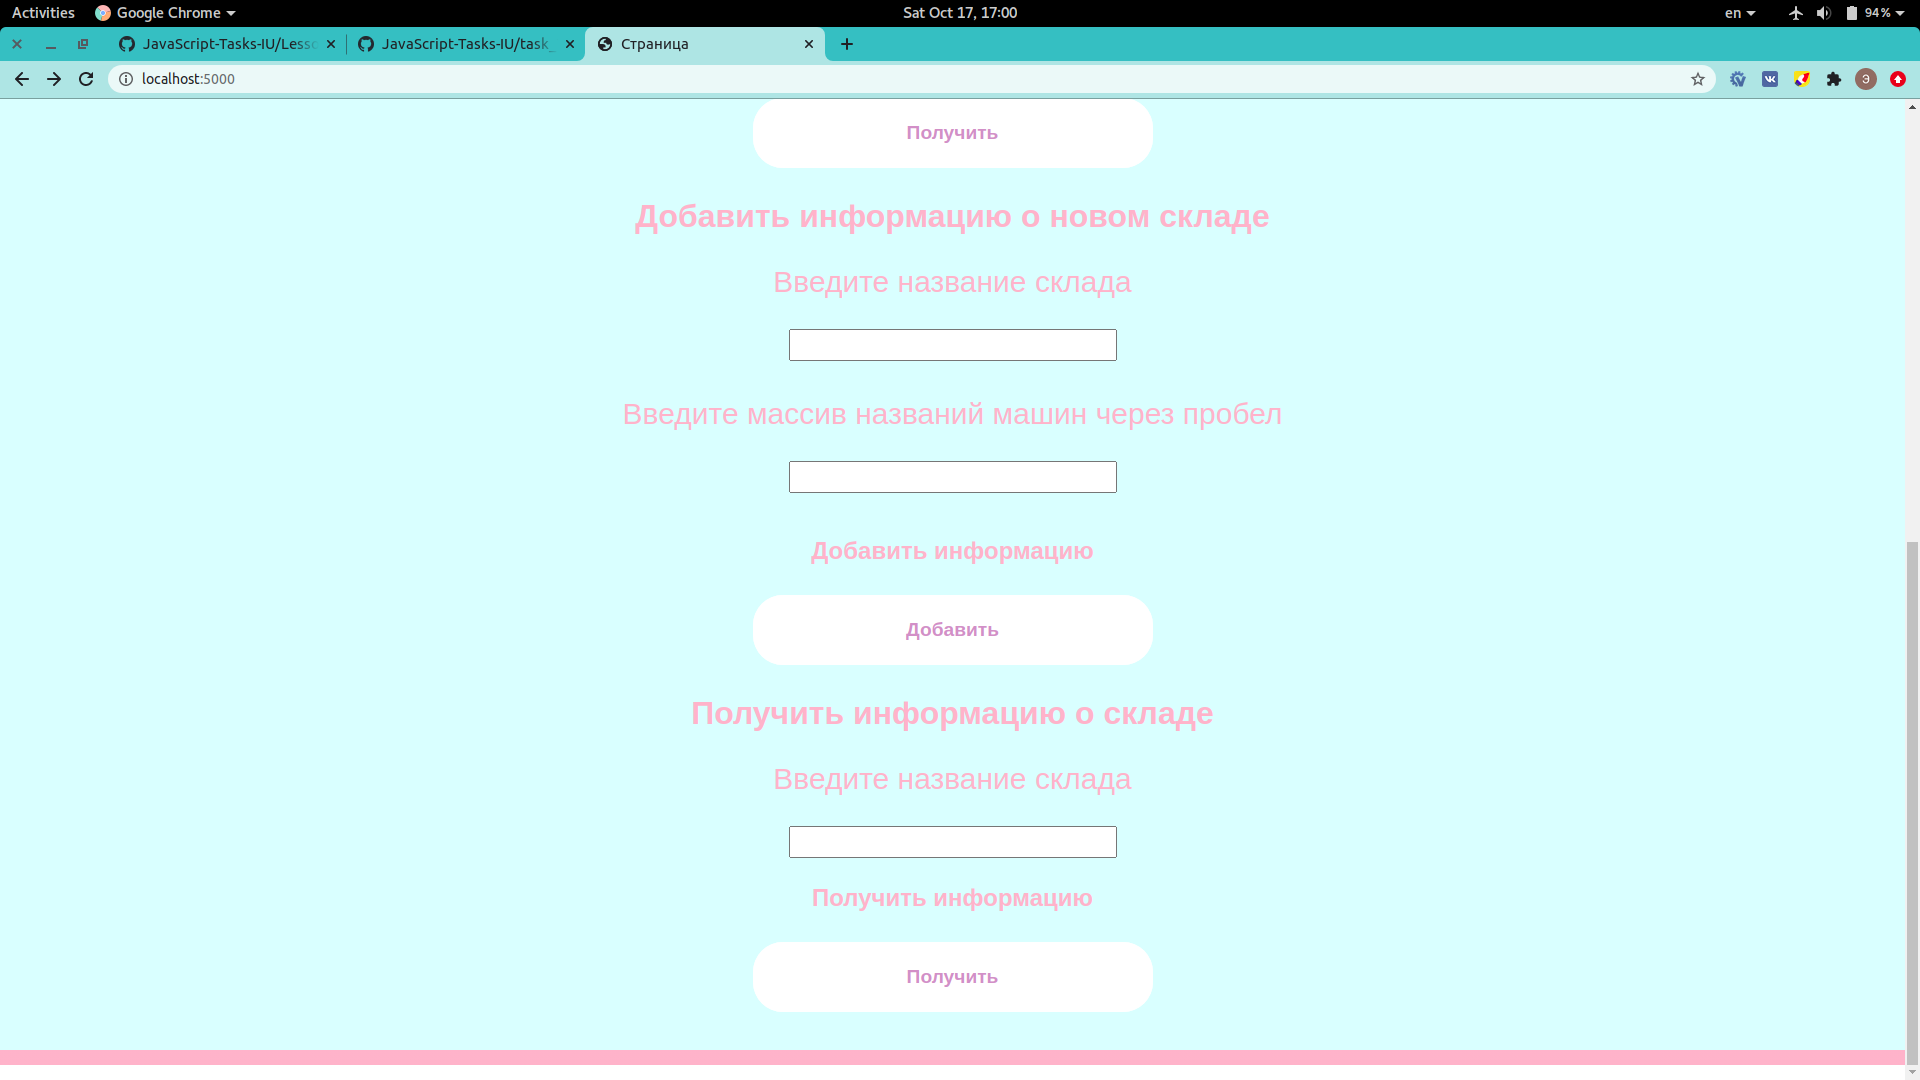
\includegraphics[width=0.9\textwidth]{img/3.png}
		\caption{Пример работы программы}}
\end{figure}


\begin{figure}[ht!]
	\centering{
		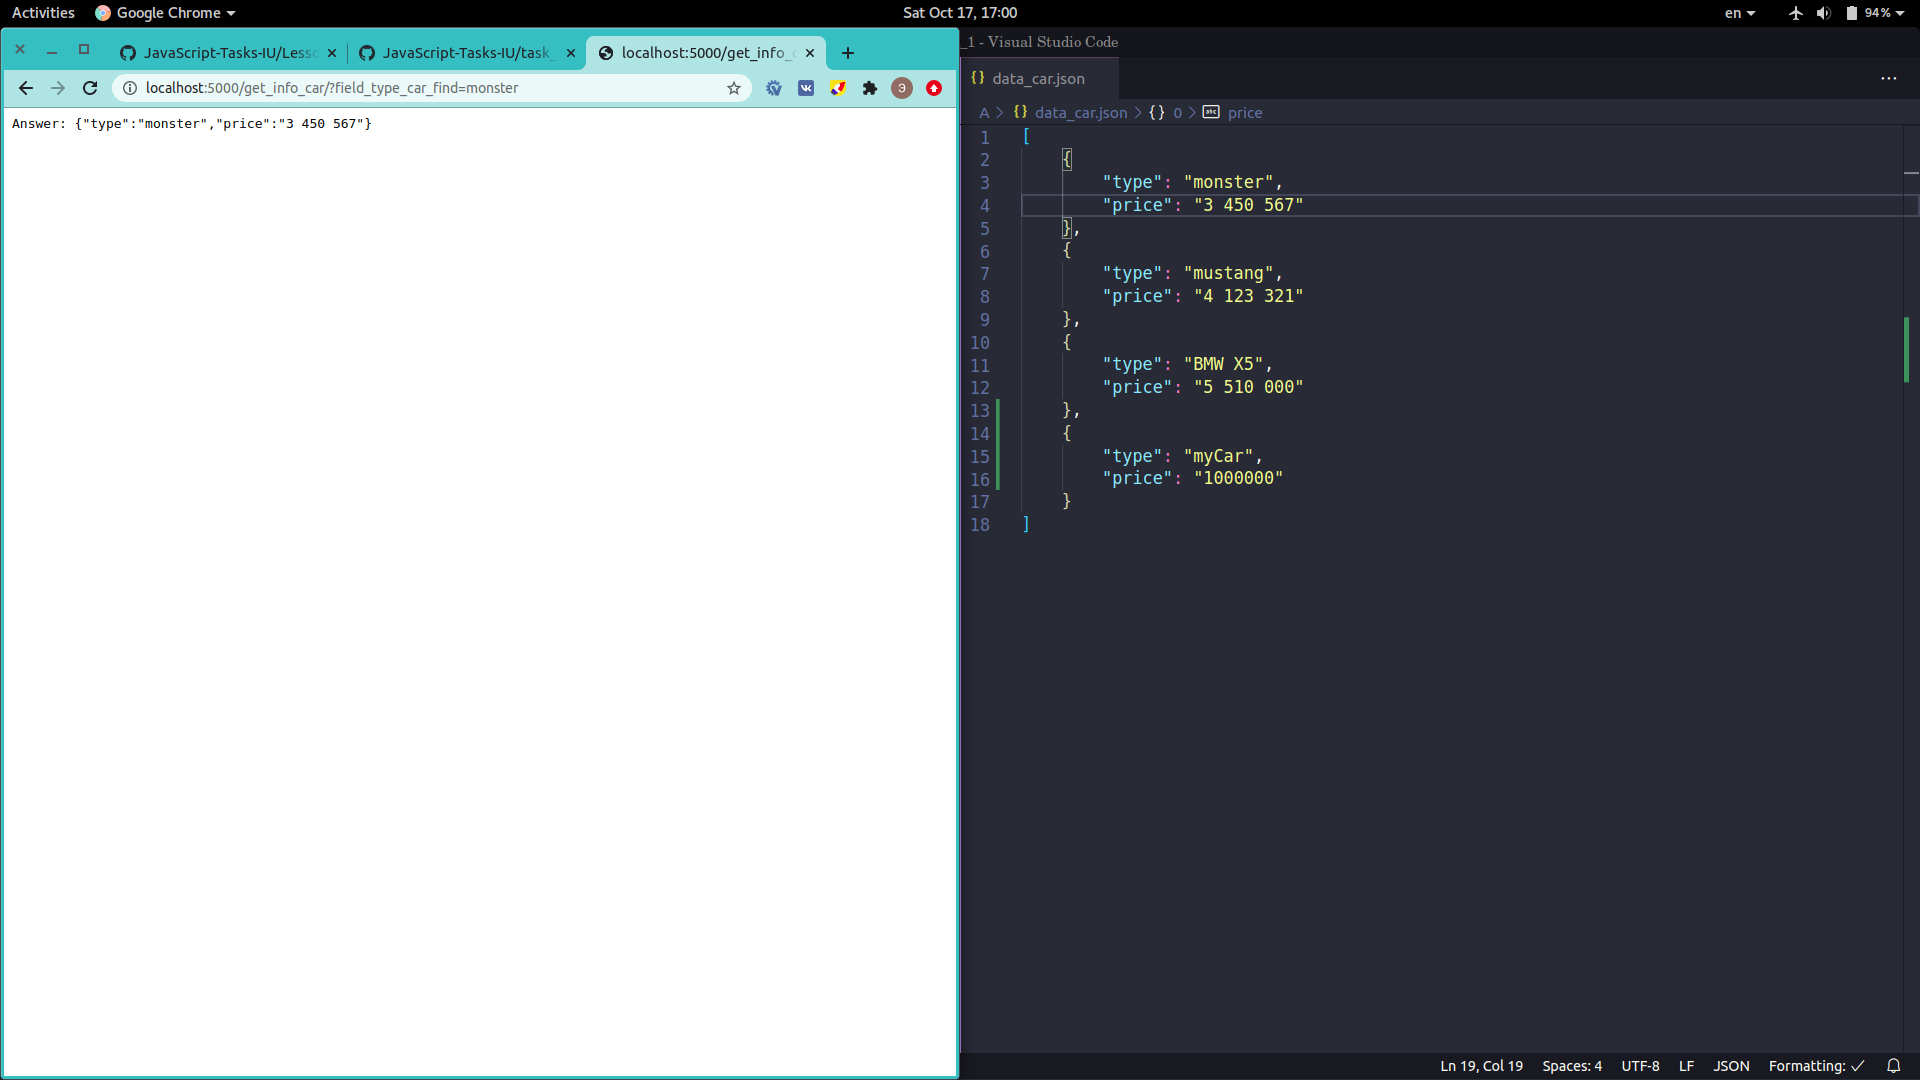
\includegraphics[width=0.9\textwidth]{img/4.png}
		\caption{Пример работы программы}}
\end{figure}


\begin{figure}[ht!]
	\centering{
		
\includegraphics[width=0.9\textwidth]{img/5.png}
		\caption{Пример работы программы}}
\end{figure}


\begin{figure}[ht!]
	\centering{
		
\includegraphics[width=0.9\textwidth]{img/6.png}
		\caption{Пример работы программы}}
\end{figure}


\begin{figure}[ht!]
	\centering{
		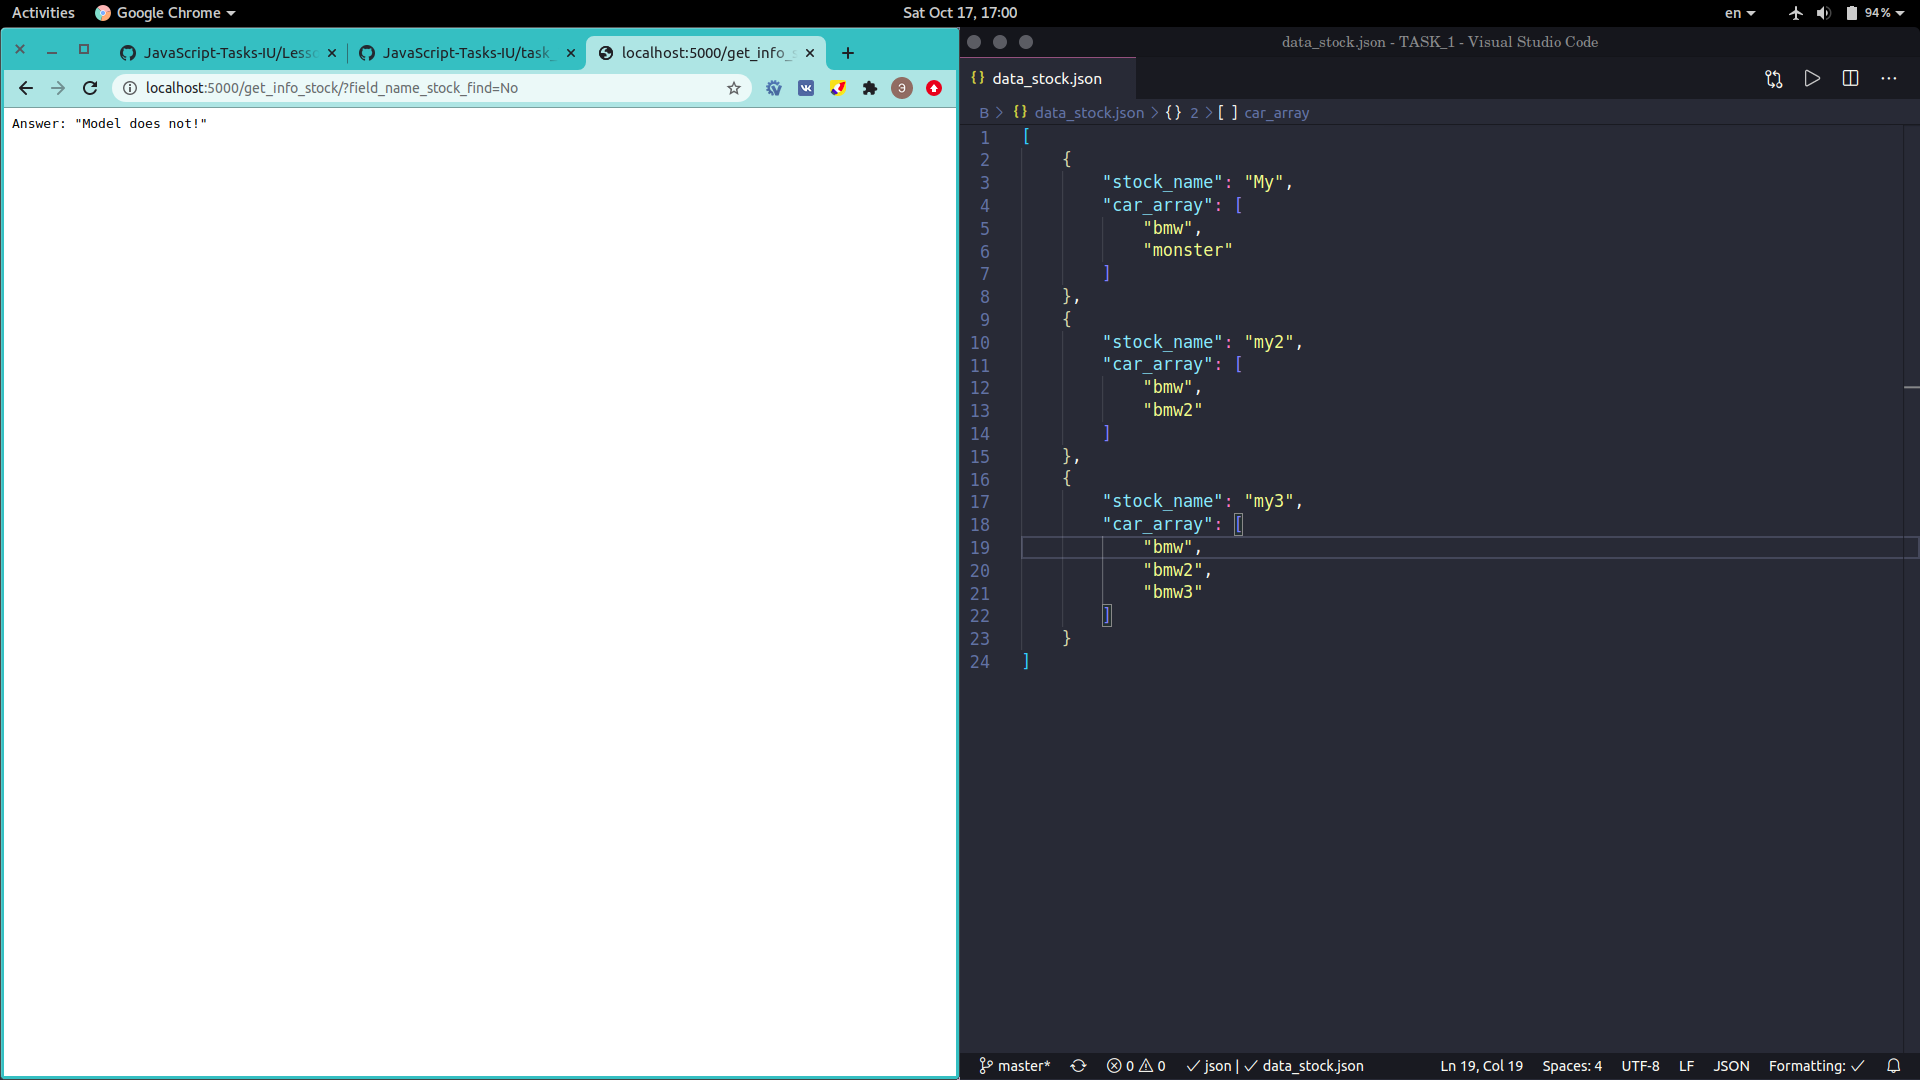
\includegraphics[width=0.9\textwidth]{img/7.png}
		\caption{Пример работы программы}}
\end{figure}

